\documentclass[usenatbib]{latex/mn2e} 
%External Packages and personalized macros
%=========================================================================
%		EXTERNAL PACKAGES
%=========================================================================
\usepackage{amsmath} 
\usepackage{amssymb} 
\usepackage {graphicx}
%\usepackage{graphics}
\usepackage[dvips]{epsfig}
\usepackage{epsfig}  
\usepackage{color}
\usepackage[normalem]{ulem}
\usepackage{hyperref}
\usepackage{caption}

%=========================================================================
%		INTERNAL MACROS
%=========================================================================
\def\be{\begin{equation}}
\def\ee{\end{equation}}
\def\ba{\begin{eqnarray}}
\def\ea{\end{eqnarray}}

% To highlight comments 
\definecolor{red}{rgb}{1,0.0,0.0}
\newcommand{\red}{\color{red}}
\definecolor{darkgreen}{rgb}{0.0,0.5,0.0}
\newcommand{\SRK}[1]{\textcolor{darkgreen}{\bf SRK: \textit{#1}}}
\newcommand{\SRKED}[1]{\textcolor{darkgreen}{\bf #1}}

\newcommand{\LCDM}{$\Lambda$CDM~}
\newcommand{\beq}{\begin{eqnarray}}  
\newcommand{\eeq}{\end{eqnarray}}  
\newcommand{\zz}{$z\sim 3$} 
\newcommand{\apj}{ApJ}  
\newcommand{\apjs}{ApJS}  
\newcommand{\apjl}{ApJL}  
\newcommand{\aj}{AJ}  
\newcommand{\mnras}{MNRAS}  
\newcommand{\mnrassub}{MNRAS accepted}  
\newcommand{\aap}{A\&A}  
\newcommand{\aaps}{A\&AS}  
\newcommand{\araa}{ARA\&A}  
\newcommand{\nat}{Nature}  
\newcommand{\physrep}{PhR}
\newcommand{\pasp}{PASP}    
\newcommand{\pasj}{PASJ}    
\newcommand{\avg}[1]{\langle{#1}\rangle}  
\newcommand{\ly}{{\ifmmode{{\rm Ly}\alpha}\else{Ly$\alpha$}\fi}}
\newcommand{\hMpc}{{\ifmmode{h^{-1}{\rm Mpc}}\else{$h^{-1}$Mpc }\fi}}  
\newcommand{\hGpc}{{\ifmmode{h^{-1}{\rm Gpc}}\else{$h^{-1}$Gpc }\fi}}  
\newcommand{\hmpc}{{\ifmmode{h^{-1}{\rm Mpc}}\else{$h^{-1}$Mpc }\fi}}  
\newcommand{\hkpc}{{\ifmmode{h^{-1}{\rm kpc}}\else{$h^{-1}$kpc }\fi}}  
\newcommand{\hMsun}{{\ifmmode{h^{-1}{\rm {M_{\odot}}}}\else{$h^{-1}{\rm{M_{\odot}}}$}\fi}}  
\newcommand{\hmsun}{{\ifmmode{h^{-1}{\rm {M_{\odot}}}}\else{$h^{-1}{\rm{M_{\odot}}}$}\fi}}  
\newcommand{\Msun}{{\ifmmode{{\rm {M_{\odot}}}}\else{${\rm{M_{\odot}}}$}\fi}}  
\newcommand{\msun}{{\ifmmode{{\rm {M_{\odot}}}}\else{${\rm{M_{\odot}}}$}\fi}}  
\newcommand{\lya}{{Lyman$\alpha$~}}
\newcommand{\clara}{{\texttt{CLARA}}~}
\newcommand{\rand}{{\ifmmode{{\mathcal{R}}}\else{${\mathcal{R}}$ }\fi}}  

%MY COMMANDS #############################################################
\newcommand{\sub}[1]{\mbox{\scriptsize{#1}}}
\newcommand{\dtot}[2]{ \frac{ d #1 }{d #2} }
\newcommand{\dpar}[2]{ \frac{ \partial #1 }{\partial #2} }
\newcommand{\pr}[1]{ \left( #1 \right) }
\newcommand{\corc}[1]{ \left[ #1 \right] }
\newcommand{\lla}[1]{ \left\{ #1 \right\} }
\newcommand{\bds}[1]{\boldsymbol{ #1 }}
\newcommand{\oiint}{\displaystyle\bigcirc\!\!\!\!\!\!\!\!\int\!\!\!\!\!\int}
\newcommand{\mathsize}[2]{\mbox{\fontsize{#1}{#1}\selectfont $#2$}}
\newcommand{\eq}[2]{\begin{equation} \label{eq:#1} #2 \end{equation}}
%#########################################################################

\begin{document}

%=========================================================================
%		FRONT MATTER
%=========================================================================
\title[LG Environment]{The place of the local group in the cosmic web}
\author[S. Bustamante and J.E. Forero-Romero]{
\parbox[t]{\textwidth}{\raggedright 
  Sebastian Bustamante \thanks{sbustama@pegasus.udea.edu.co}$^{1}$ 
  Jaime E. Forero-Romero$^{2}$ 
}
\vspace*{6pt}\\
$^1$Instituto de F\'{\i}sica - FCEN, Universidad de Antioquia, Calle
67 No. 53-108, Medell\'{\i}n, Colombia\\ 
$^2$Departamento de F\'{i}sica, Universidad de los Andes, Cra. 1
No. 18A-10, Edificio Ip, Bogot\'a, Colombia
}

\maketitle

\begin{abstract}


We present a theoretical study Local Group in a cosmological context. 
The principal objective is to find a coherent sample of LG systems in 
the unconstrained simulation Bolshoi based upon the properties of hand 
construted LG systems in the constrained simulations CLUES. We obtain a 
privileged environment for these systems and significant bias in some of 
their properties. (\SRKED{draft!})

\end{abstract}

\begin{keywords}
galaxies: high-redshift - galaxies: star formation - line: formation
\end{keywords}


%=========================================================================
%		PAPER CONTENT
%=========================================================================

%*************************************************************************
\section{Introduction}
\label{sec:introduction}
%*************************************************************************


The spatial distribution of galaxies describes a web-like pattern, the 
so-called cosmic web. Today it is understood that such configuration is 
driven by gravitational instabilities. ...



The study of the influence of the cosmic web on galaxy properties start 
with the seminal work of Dressler \SRKED{[reference here]} and extends to 
recent works using large observational surveys that look for signatures of 
the web into the evolution of galaxy populations. With the advention of 
more detailed observations and sophisticated computational models it is 
now within our reach to understand what physical processes dominate.



This makes  that the mass assembly history of a galaxy is deeply connected 
with its  position in the cosmic web. There is an extensive body of 
literature on the effects of the web environment on the observable 
properties of galaxies. 



This environmental study is also of paramount importance to understand the 
formation of our Galaxy. In our local neighborhood, the observations of 
dwarf galaxies around the Milky Way (MW) and the Andromeda galaxy (M31) 
show filamentary and disk-like patterns that can be linked to a 
preferential infall direction, very likely connected with the cosmic web 
where the Local Group (LG) of galaxies is embedded. 



In this paper we quantify the velocity shear environment of DM halo pairs
representative of the principal members of the Local Group (LG), the Milky
Way (MW) and Andromeda galaxy (M31). We perform this study in an 
unconstrained cosmological simulation from random phases in the initial 
conditions, and unlike previous works, where were used constrained 
cosmological simulations which have been setup as to reproduce the large 
scale structure of the local universe, we use directly observational 
measurements of the kinematics properties of the local group \SRKED{
[Reference here]} in order to build faithful samples of LG-like systems.



We pay special attention to the correlation of the present velocity shear 
environment with the assembly and the kinematics properties of the pairs. 
The motivation to have that focus is that it has been previously shown 
that the LG present in three different realizations of the constrained 
simulations have assembly histories biased towards early formation times 
and absence of major mergers (ratio 1:10) in the last $10$ Gyr. In the 
case of the kinematic properties, recent observational constrains to the 
galactocentric tangential velocity of M31 has enabled to establish how 
typical is the LG in a cosmological context \SRKED{[reference to 
Forero-Romero 2013-1]}, that is why we focus here how a specific kind of 
host environment biases these kinematics properties.



%*************************************************************************
\section{The Simulation}
\label{sec:the_simulation}
%*************************************************************************


As it was previously mentioned, we use an unconstrained cosmological 
simulation, the Bolshoi simulation, to identify the possible large scale 
environment of the Local Group. This is a similar approach to the one already 
used by \SRKED{[reference here]}.



The Bolshoi simulations follows the non-linear evolution of a dark matter 
density field on a cubic volume of size $250$\hMpc sampled with $2048^3$ 
particles. The cosmological parameters in the simulation are 
$\Omega_{\rm m}=0.27$, $\Omega_{\Lambda}=0.73$, $h=0.70$, $n=0.95$ and 
$\sigma_{8}=0.82$ for the matter density, cosmological constant, 
dimensionless Hubble parameter, spectral index of primordial density 
perturbations and normalization for the power spectrum. The mass of each 
particle in the simulation is $m_{\rm p}=1.4\times 10^{8}$\hMsun.



%-------------------------------------------------------------------------
\subsection{Halos and Merger Trees}
\label{subsec:halos_merger_trees}
%-------------------------------------------------------------------------



We identify halos with two algorithms, the Friends-of-Friends \SRKED{
[reference here]} algorithm and the Bound Density Maximum algorithm. The 
constructed catalogues also provide the basis for the mass aggregation 
history studies. We also include in the catalogues information about the 
substructure.



All the results presented here must be interpreted in term of host halos, 
without any information of the substructure. In particular the merger of 
two FOF halos corresponds to the epoch of first overlap, and not to the 
fusion and/or disruption of an accreted sub-halo with a dominant halo. 



The linking length is $b=0.17$ times the mean inter-particle separation. 
All objects with 20 particles or more are considered a bona fide halo and 
are included in the construction of the merger tree, this corresponds to a 
minimum halo mass of $M_{\rm min}=3.78\times 10^{8}$ \hMsun in the CLUES 
volumes and $M_{\rm min}=2.70\times 10^{9}$\hMsun in the Bolshoi 
simulation.



The halo identification for the CLUES simulation was done for 80 snapshots
in the redshift range $0<z<7$ more or less evenly spaced in look-back time. 
For Bolshoi we use the information of XX snapshots in the same redshift 
ssrange.



%*************************************************************************
\section{Algorithms to quantify the cosmic environment}
\label{sec:algorithms_cosmic_web}
%*************************************************************************



%-------------------------------------------------------------------------
\subsection{The tidal web - T-web}
\label{subsec:Tweb}
%-------------------------------------------------------------------------



The first algorithm  we use to identify the cosmic web is based on the
diagonalization of the tidal tensor, defined as the Hessian of a 
normalized gravitational potential  


%.........................................................................
%Tidal Tensor
\begin{equation}
T_{\alpha\beta} = \frac{\partial^2\phi}{\partial x_{\alpha}\partial x_{\beta}}
\end{equation}
%.........................................................................
where the physical gravitational potential has been rescaled by a factor 
$4\pi G\bar{\rho}$ in such a way that $\phi$ satisfies the following 
equation



%.........................................................................
%Poisson
\begin{equation}
\nabla^2\phi = \delta,
\end{equation}
%.........................................................................
where $\bar{\rho}$ is the average density in the Universe, $G$ is the 
gravitational constant and $\delta$ is the dimensionless matter 
overdensity.



%-------------------------------------------------------------------------
\subsection{The velocity  web - V-web}
\label{sec:Vweb}
%-------------------------------------------------------------------------



We use the a kinematical method to define the cosmic-web environment in 
the simulation. The method has been thoroughly described in XXX and 
applied to study the shape and spin alignment in the Bolshoi simulation 
here XX. We refer the reader to these papers to find a detailed 
description of the algorithm, its limitations and capabilities. Here we 
summarize the most relevant points for the discussion. 



The V-web method for environment finding is based on the local shear 
tensor calculated from the smoothed DM velocity field in the simulation.
The central quantity is the following dimensionless quantity 


%.........................................................................
%V-Web Definition
\eq{V_web}
{
\Sigma_{\alpha\beta} = -\frac{1}{2H_0}\pr{\frac{\partial v_{\alpha}}
{\partial x_{\beta}}+\frac{\partial v_{\beta}}{\partial x_{\alpha}}}
}
%.........................................................................
where $v_{\alpha}$ and $x_{\alpha}$ represent the $\alpha$ component of 
the comoving velocity and position, respectively. $\Sigma_{\alpha\beta}$ 
can be represented by a $3\times 3$ symmetric matrix with real values,
that ensures that is possible to diagonalize and obtain three real 
eigenvalues $\lambda_{1} > \lambda_{2}>\lambda_3$ whose sum (the trace of
$\Sigma_{\alpha\beta}$) is proportional to the divergence of the local 
velocity field smoothed on the physical scale ${\mathcal R}$. 



The relative strength of the three eigenvalues with respect to a threshold
values $\lambda_{th}$ allows for the local classification of the matter 
distribution into four web types. Voids, sheets, filaments and peaks, 
which correspond to regions with 3, 2, 1 or 0 eigenvalues with values 
larger than $\lambda_{th}$. In this paper we do not perform an definitive 
classification into web types, instead we express the results respect to 
the relative strength of the eigenvalues and in a range of $\lambda_{th}$.
We consider \textit{a posteriori} the possible web type interpretation 
that could be feasible within a range of thresholds for the eigenvalues. 



%-------------------------------------------------------------------------
\subsection{The Web in Bolshoi}
\label{subsec:web_in_simulations}
%-------------------------------------------------------------------------
... Resolution and Smoothing

... Database


%-------------------------------------------------------------------------
\subsection{Method to find void regions}
\label{subsec:method_voids}
%-------------------------------------------------------------------------



Following the recent work of \SRKED{Courtois et al. 2013}, we use a method 
based on a FOF algorithm to find extended regions of voids and then, we 
select halo systems according to a proximity criteria to those regions. 
In order to perform this, we build the input FOF catalogue with the 
positions of the center coordinate of every cell marked as void according 
to the web scheme adopted; furthermore we set an adequate linking length 
for connecting diagonal neighbour cells.



Following the work of \SRKED{Forero-Romero et al. 2008}, we also perform a 
percolation analysis in order to select the best threshold parameter that
reduce percolation in cells, thereby accounting for physical voids regions.



%*************************************************************************
\section{Local Group Sample Definition}
\label{section:Def_Samples}
%*************************************************************************



In order to establish an adequate set of criteria to define LG samples in 
unconstrained simulations, we proceed from the the general dark halo 
catalogues, constructed using the FOF scheme with a linking length of 
$b=0.17$. These samples are defined for all simulation and will be 
referred as General Halos (GH) samples. To be consistent with the 
observationally determined mass range of halos that host disk-form 
galaxies, we select the halos in the mass range $5\times10^{11} <
M_{h}/\hMsun < 5\times 10^{12}$, referred here as Individual Halos (IH) 
samples. 



As a primal approach to define gravitational bounded halo pairs we select 
all halo pairs in IH samples that satisfied to be the closest to each 
other, they constitute the Pairs (P) samples. To keep the concordance with
previous works in algorithms for LG selection (\SRKED{[references here}), 
we define here the next list of conditions that have to fulfill a pair 
system in order to construct the Isolated Pairs (IP) samples. All these 
considerations are based upon the relative dynamics of the Milky Way and 
M31, and its isolation from massive structures:



%.........................................................................
%Isolated pairs criteria
\begin{enumerate}

\item{The distance between the center of the two halos should be less than 
$0.7$\hMpc.}

\item{The relative physical velocity between the two halos has to be 
negative.}

\item{The distance to any halo more massive than any of the pair members 
must be less than $2$\hMpc.}

\item{The distance to cluster-like halos with masses larger than 
$1\times10^{13}$ \hMsun must be larger than $5$\hMpc.}
\end{enumerate}
%.........................................................................


In the case of a constrained simulation one can define samples of LG 
systems based upon the next condition


%.........................................................................
%Additional criteria
\begin{enumerate}
\item[(v)]{The Local Group pair must be located in the right environment 
with respect to the XX Cluster.}
\end{enumerate}
%.........................................................................

%.........................................................................
%Table of extreme values of LG environment
\begin{table}
  \centering
  \begin{tabular}{l | c c c} \hline
	& $\bds{\lambda_{1}}\ [10^{-1}]$ & $\bds{\lambda_{2}}\ [10^{-1}]$  & $\bds{\lambda_{3}}\ [10^{-1}]$ \\ \hline
	\textbf{Minim value} & 1.78 & -6.29$\times 10^{-2}$ & -1.98 \\
	\textbf{Maxim value} & 3.49 & 1.21 & -8.85$\times 10^{-1}$ \\ \hline
  \end{tabular}
  
  \caption{Extreme values for each V-web eigenvalues to construct LG 
  samples.}
  
  \label{Tab:Lambdas_LG}
\end{table}
%.........................................................................



Due to the intrinsic nature of constrained simulations, we expect that 
these LG samples be the most faithful systems that resemble the properties
and the environment of our LG. In fact, the three CLUES simulations appear 
to present a common V-web/T-web environment for LG systems, such as shown 
in the figure \ref{fig:LG_CLUES_Environment}. Based in this we propose a 
new criteria of selection to define more realistic LG systems in the
unconstrained simulation, this consists in tanking the extreme values of 
each V-web/T-web eigenvalue associated to the host environment of the three 
LG systems in CLUES. With this range established (see table 
\ref{Tab:Lambdas_LG}) we filter the IP sample in Bolshoi simulation in 
order to build the samples Constructed Local Groups V-web based (CLGV) 
and T-web based (CLGT). Finally in the table \ref{Tab:Samples_Size} we 
show the sizes of all defined samples for each simulation.



%.........................................................................
% Environment of LG in each CLUES simulation
\begin{figure*}
\begin{center}
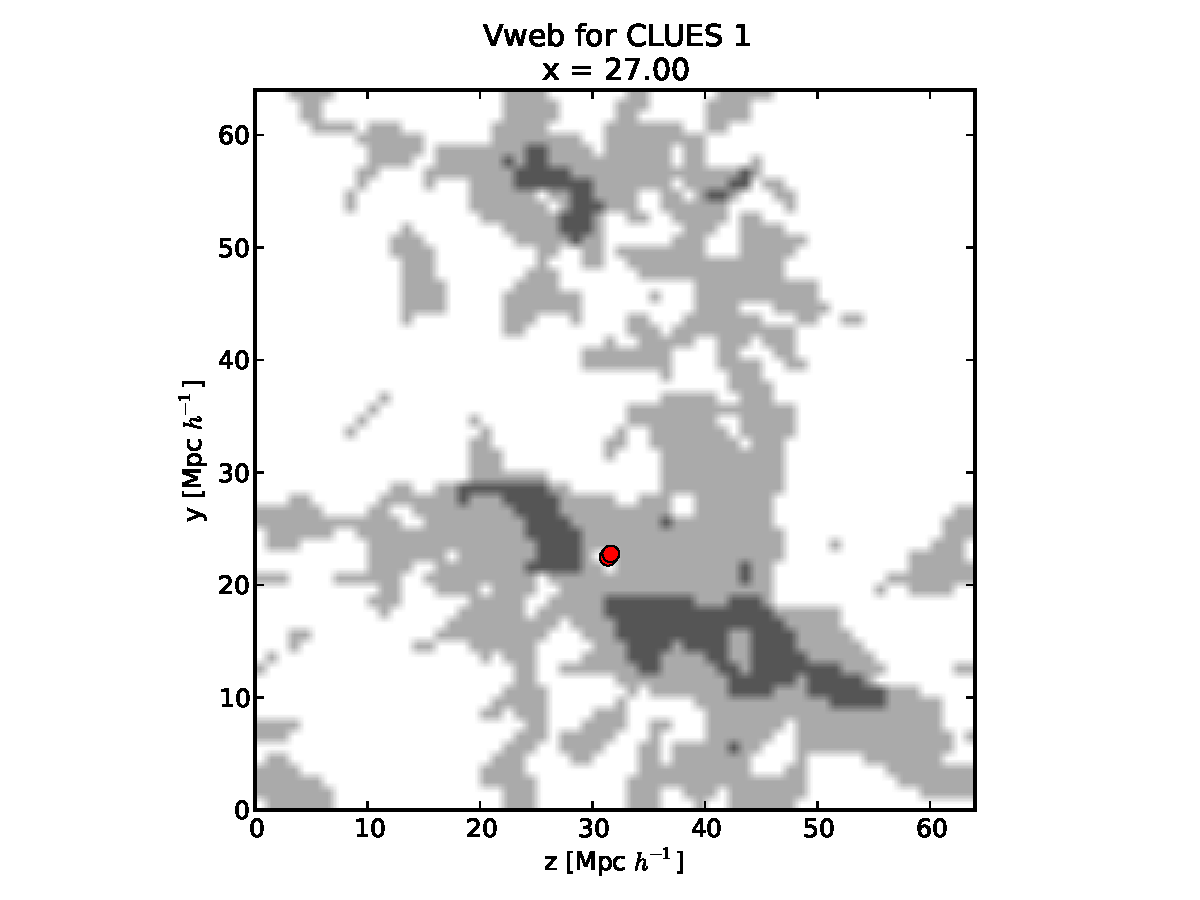
\includegraphics[trim = 30mm 0mm 35mm 0mm, clip, keepaspectratio=true,
width=0.2\textheight]{./figures/LG_C1_Env_Vweb.pdf}
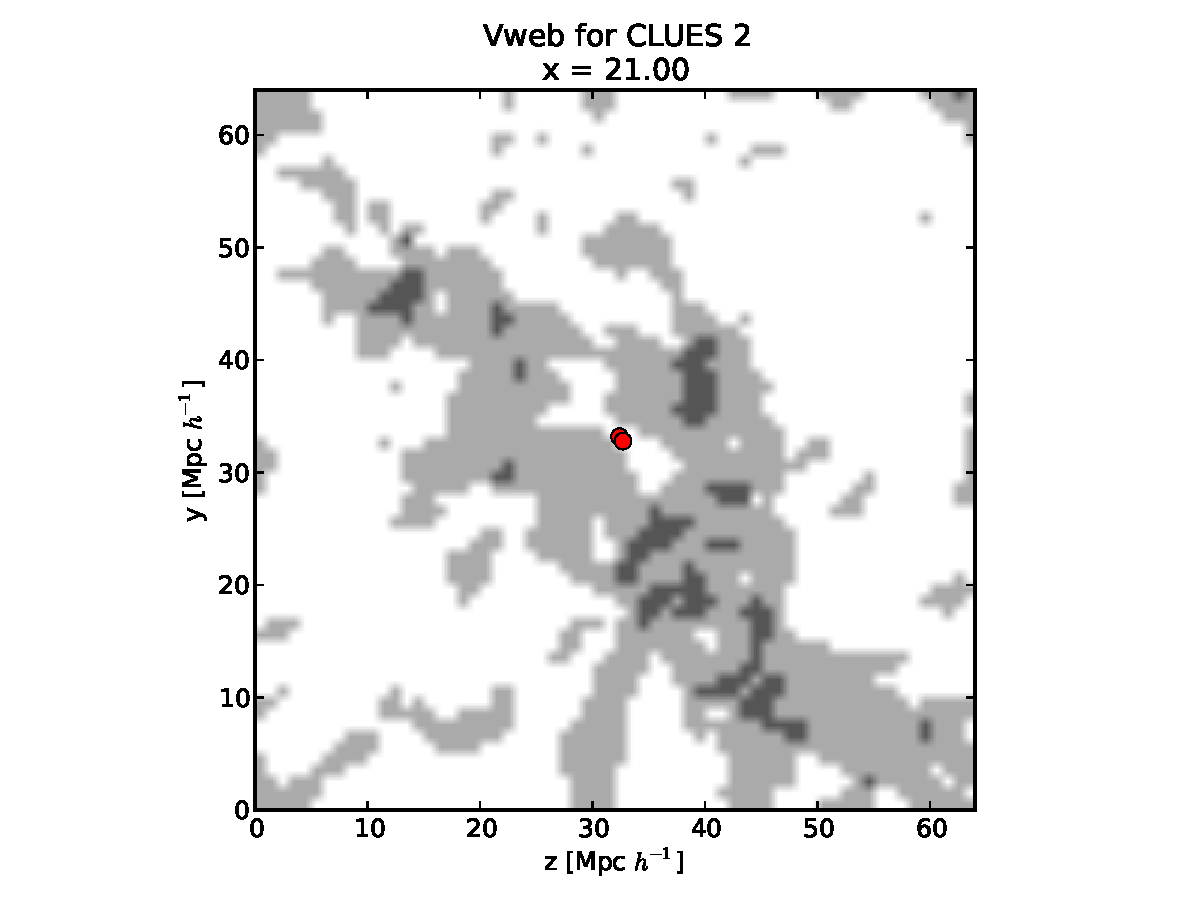
\includegraphics[trim = 30mm 0mm 35mm 0mm, clip, keepaspectratio=true,
width=0.2\textheight]{./figures/LG_C2_Env_Vweb.pdf}
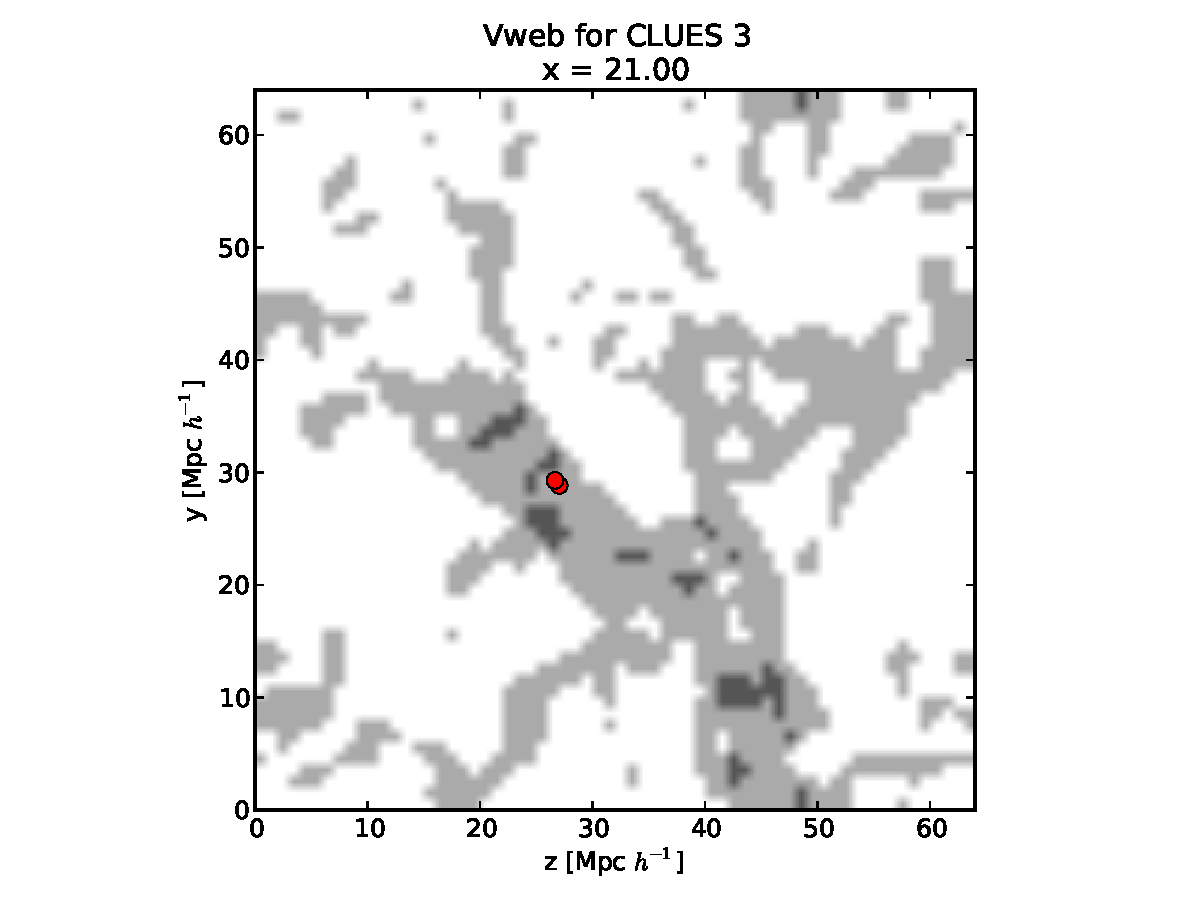
\includegraphics[trim = 30mm 0mm 35mm 0mm, clip, keepaspectratio=true,
width=0.2\textheight]{./figures/LG_C3_Env_Vweb.pdf}

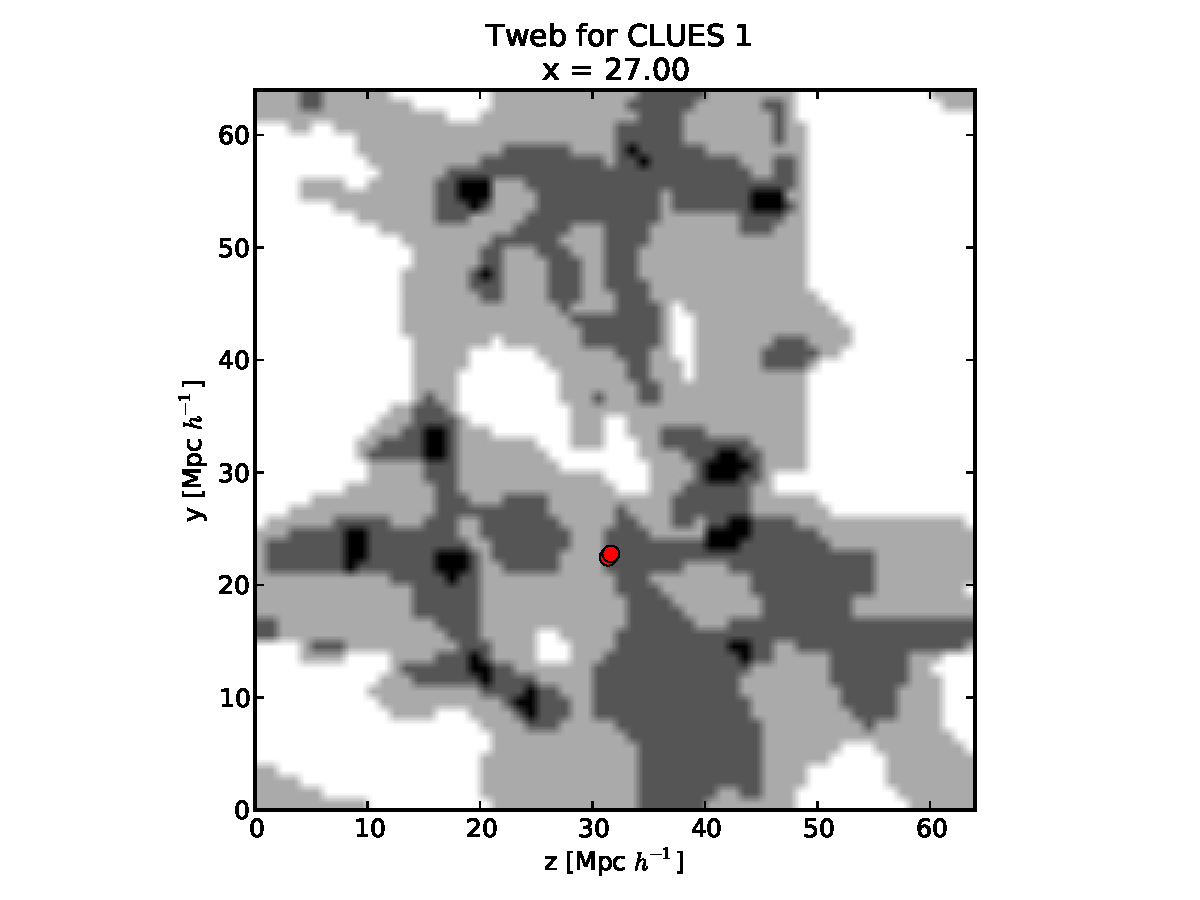
\includegraphics[trim = 30mm 0mm 35mm 0mm, clip, keepaspectratio=true,
width=0.2\textheight]{./figures/LG_C1_Env_Tweb.pdf}
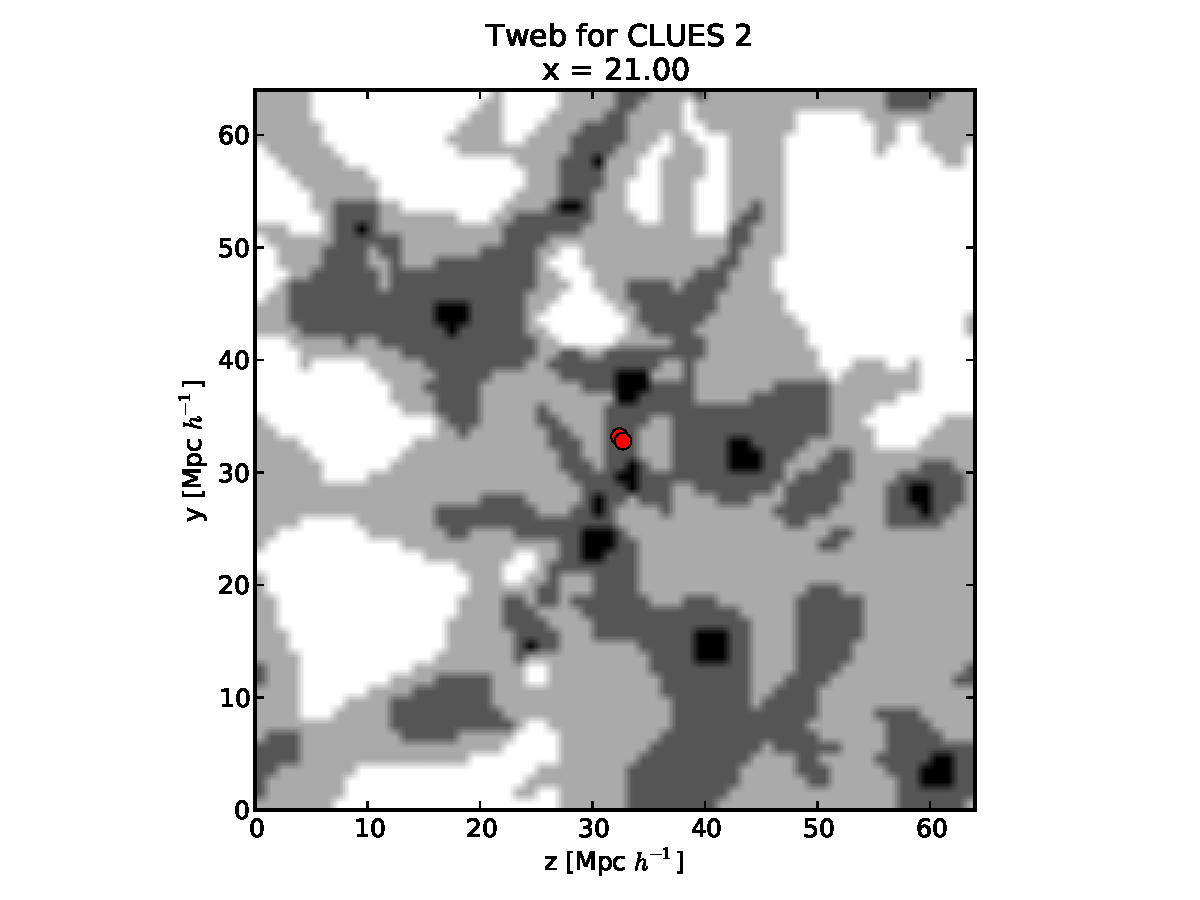
\includegraphics[trim = 30mm 0mm 35mm 0mm, clip, keepaspectratio=true,
width=0.2\textheight]{./figures/LG_C2_Env_Tweb.pdf}
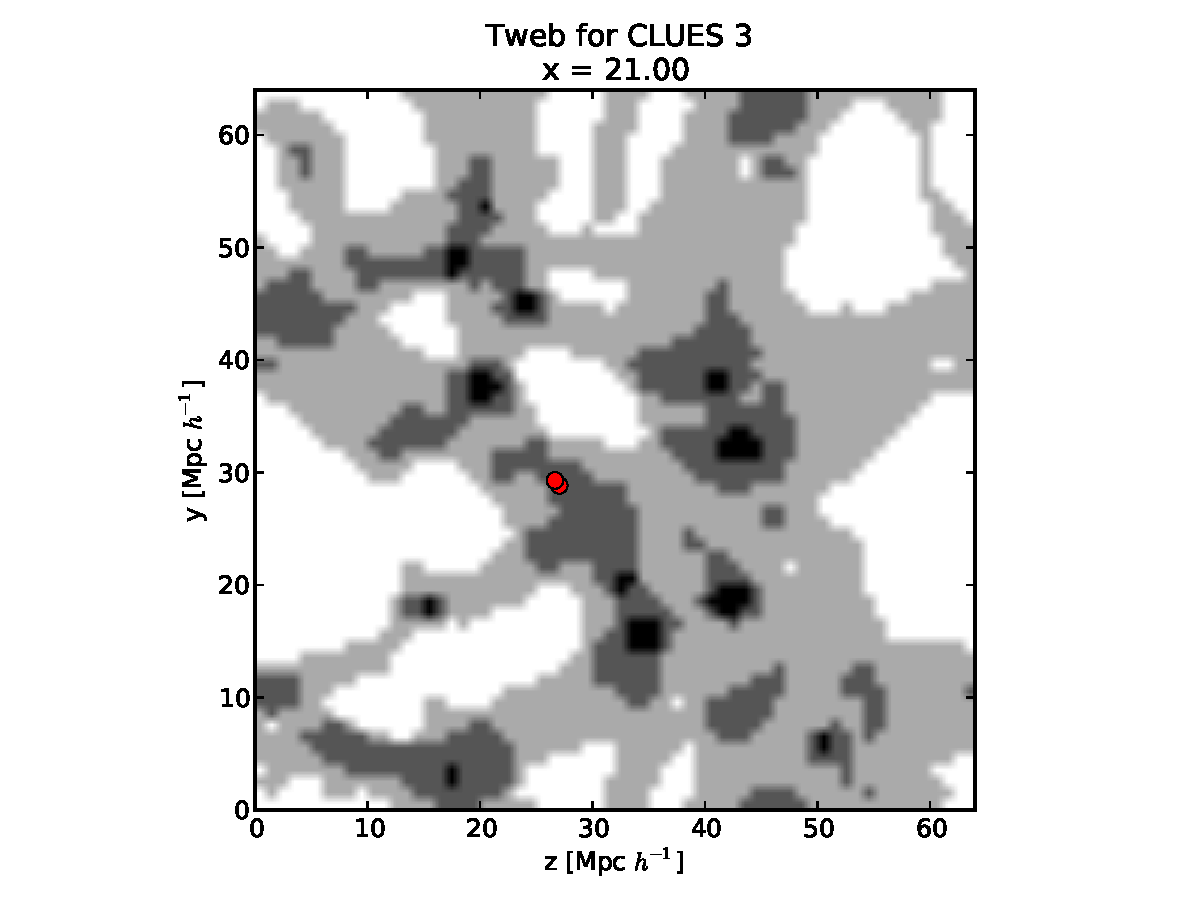
\includegraphics[trim = 30mm 0mm 35mm 0mm, clip, keepaspectratio=true,
width=0.2\textheight]{./figures/LG_C3_Env_Tweb.pdf}

\caption{\small Environment of LG systems in each CLUES simulation, 
according to V-web scheme (upper figures) and to T-web scheme (lower 
figures). In both cases we use a threshold value of $\lambda_{th}^{V/T} = 
0.25$.}
\label{fig:LG_CLUES_Environment}
\vspace{0.1 cm}
\end{center}
\end{figure*}
%.........................................................................

%.........................................................................
%Table of samples numbers
\begin{table}
  \centering
  \begin{tabular}{l | c c c c} \hline
	\textbf{Sample}& \textbf{CLUES} & \textbf{CLUES} & \textbf{CLUES} & \textbf{Bolshoi} \\
	\textbf{description}& \textbf{1} & \textbf{2} & \textbf{3} &  \\ \hline
	GH	&	56632	&	57707	&	56799	&	432000 	\\
	IH	&	1493	&	1490	&	1493	&	88068 	\\
	P	&	386 	&	380 	&	387		&	23037 	\\
	IP	&	20	 	&	12		&	18		&	1256 	\\
	LG	&	1 		&	1 		&	1		&	-- 		\\
	CLGV &	1		&	2		&	3		&	30		\\
	CLGT &	1		&	1		&	1		&	0		\\ \hline
  \end{tabular}
  
  \caption{Size of the samples in each simulation. The relation between 
  the size of the samples scales as the relation between the volumes of 
  each respective simulation, approximately $1/60$ for the CLUES 
  simulations respect to Bolshoi.}
  
  \label{Tab:Samples_Size}
\end{table}
%.........................................................................


%*************************************************************************
\section{Finding a Local Group environment}
\label{sec:experiments}
%*************************************************************************



In this section we prepare some numerical experiments with the halos 
samples and their environment, with special emphasis on the isolated pairs 
and LG samples. All this in order to find for environment correlations and 
common properties between LG systems.


%-------------------------------------------------------------------------
\subsection{Comparison of the two simulations}
\label{subsec:comparison_simulations}
%-------------------------------------------------------------------------


Prior to study of isolated and LG samples and to determinate possible 
correlations between their properties, it is necessary to establish the 
equivalence between all simulations that we will use, with the aim to 
eliminate effects due to construction process of each one.


In first place, we analyse the mass distribution of individual halos and 
in next figure we show the integrated mass function (IMF) for halos sample
with $M \geq 1\times 10^{11} M_{\odot}$.


%.........................................................................
%IMF halos
\begin{flushleft}
\begin{center}

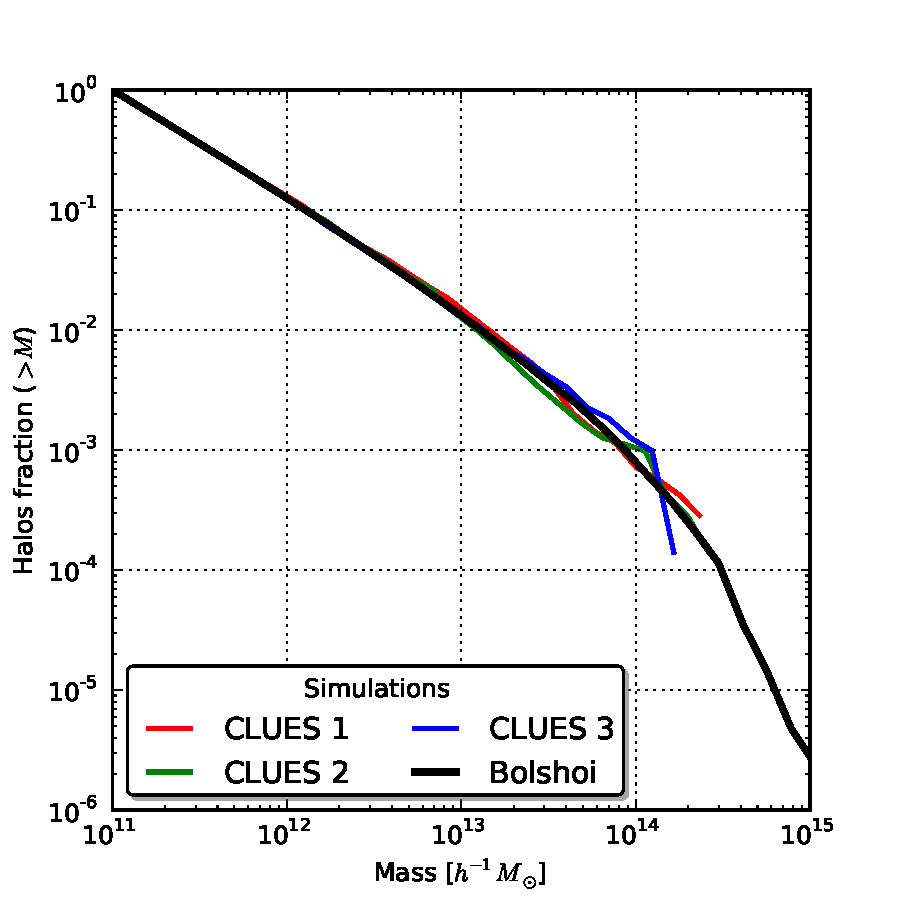
\includegraphics[keepaspectratio=true,width=0.35\textheight]
{./figures/Halos_IMF.pdf}

\captionof{figure}{\small Integrated mass function of individual halos of 
each simulation used. In the center-left, with vertical dot lines, the 
individual masses of each LG system in CLUES simulations are represented.}

\label{fig:IMF_Halos}
\vspace{0.1 cm}
\end{center}
\end{flushleft}
%.........................................................................



Although in high masses the IMF of each simulation are slightly different, 
in low mass region, where the most halos of our interest are, the IMFs are 
quite similar indicating that the sample of halos in each simulation have 
the same mass distribution, while the small differences are due to finite 
size of samples. Another aspect in the figure \ref{fig:IMF_Halos} is the 
position of LG halos, they are distributed across the mass range of halos 
that we have set (see in section \ref{section:Def_Samples}), indicating 
that there is not an apparent condition with their individual masses.



The situation is quite different respect to mass ratio index of isolated 
pairs sample (MRI). In the figure \ref{fig:Index_Pairs} (a) we show the 
integrated distribution of MRI, where the approximately linear behaviour 
indicates an uniformly distribution. The interesting aspect here is the 
closeness between the LG sample values, indicating a possible common 
property in these systems, even though this could be established a priori 
by construction. In the \ref{fig:Index_Pairs} (b) is plotted the 
integrated distribution of total pair mass, and again like the IMF, there 
is not a preferential value.



Once established the concordance between the defined samples, we proceed 
to analyse the distribution of the eigenvalue of shear velocity tensor 
\ref{eq:V_web}, for this we assume that the halos are good tracers of the 
environment properties and therefore we evaluate each eigenvalue in the 
center mass of each halo, mapping of this way the complete distribution 
(figure \ref{fig:lambda_histogram}). The black curves correspond to the 
unconstrained simulation (Bolshoi) and the color curves to the constrained 
simulations (CLUES), aditionally we calculate the cosmic variance, showed 
in purple curves, dividing the Bolshoi volume in smaller parts with a size 
comparable to the CLUES volume ($64 h^{-1 }$ Mpc of side). What is 
interesting here is the clear difference between the eigenvalues 
distributions of the both types of simulations, inclusively the 
constrained distributions does not match between the cosmic variance, 
indicating that although both simulations were made with the same cosmology 
(see subsections \ref{subsec:CLUES_simulations} and 
\ref{subsec:Bolshoi_simulation}), the constrained simulations have a 
significantly different environment properties (spatial matter distribution) 
compared to the average expected from a random volume with the same 
comoving size.


%.........................................................................
% Lambda Histogram
\begin{figure*}
\begin{center}
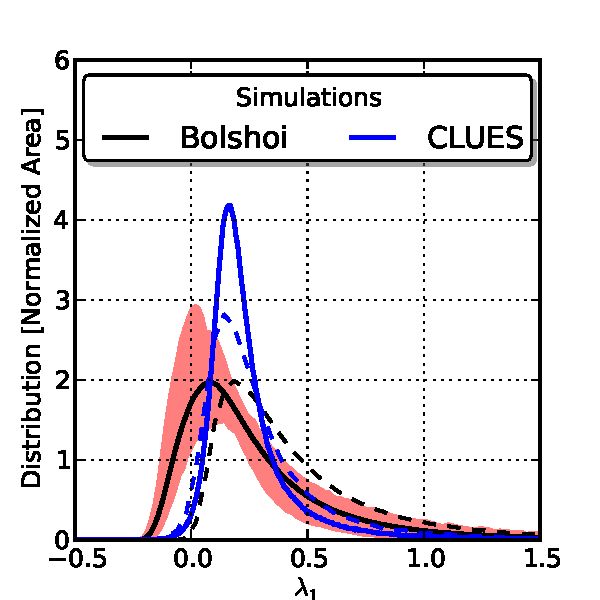
\includegraphics[trim = 0mm 0mm 5mm 8mm, clip, keepaspectratio=true,
width=0.24\textheight]{./figures/Cells_Distro_L1.pdf}
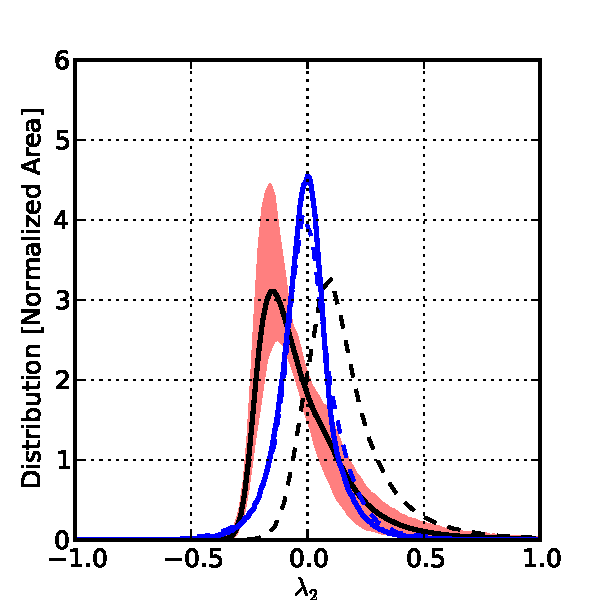
\includegraphics[trim = 0mm 0mm 5mm 8mm, clip, keepaspectratio=true,
width=0.24\textheight]{./figures/Cells_Distro_L2.pdf}
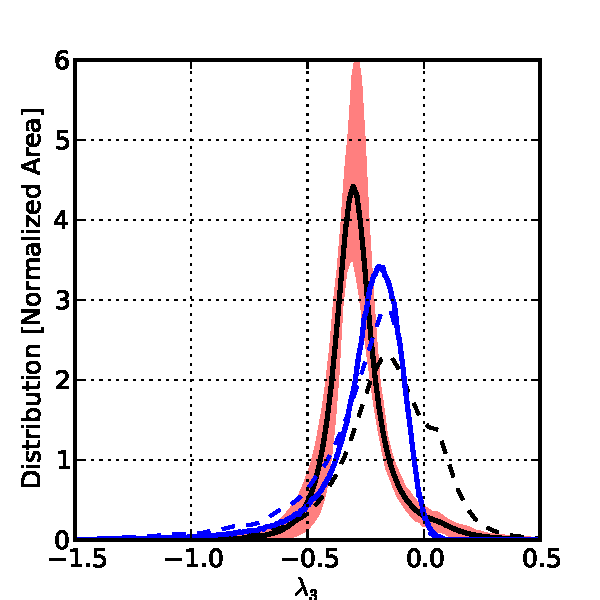
\includegraphics[trim = 0mm 0mm 5mm 8mm, clip, keepaspectratio=true,
width=0.24\textheight]{./figures/Cells_Distro_L3.pdf}

\caption{\small Integrated distribution of mass ratio index for isolated 
pairs sample (a).}

\label{fig:lambda_histogram}

\vspace{0.1 cm}
\end{center}
\end{figure*}
%.........................................................................


%-------------------------------------------------------------------------
\subsection{Defining the LG environment}
\label{subsec:LG_construction}
%-------------------------------------------------------------------------


With the aim of constructing a sample of LG systems in Bolshoi simulations, 
we use the eigenvalues of the three LG systems in each CLUES simulation 
and choose a range for each one based in the extreme values of the six 
halos, this with the expectation of reproducing the LG specific conditions 
in constrained simulations. This criteria can be thought as a first 
approximation to establish a more faithful sub-sample into the isolated 
pairs. In table \ref{Tab:Lambdas_LG} we show the used extreme values for 
each eigenvalue of local shear tensor.



As a self-consistency test, we apply this criteria to CLUES simulations 
and find, on average, three LG systems in each one. But to avoid confusion, 
we keep defining the LG sample as the three initial pairs. Finally, we 
construct the LG sample of Bolshoi, where the sample size is illustrated 
in Table \ref{Tab:Samples}.



Once we have established the equivalence of samples in each simulation and 
have defined the LG samples, we proceed to calculate correlations between 
halo samples and their environment. As was mentioned in section 
\ref{sec:Vweb}, we do not use an specific value of eigenvalue threshold 
$\lambda_{th}$, instead of this, we explore a relatively wide range of 
this parameter (i.e. $0 \leq \lambda_{th} \leq 1$) and calculate 
distributions respect to each eigenvalue individually.



At first place, we calculate the environment of each LG system in CLUES 
simulations, for this we use the $\lambda_{th}$ scheme to classify it in 
void, sheet, filament or knot (see \ref{sec:Vweb}), with $\lambda_{th}$
into the threshold range. Figure \ref{fig:LG_Env_CLUES} is obtained.



At first place, we calculate the integrated distribution of each 
eigenvalue for individual halos, isolated pairs and LG samples. For this, 
we associate to each halo a value of environment (set of eigenvalues)
according to its center of mass position in a smoothed grid ($256^3$ 
cells for Bolshoi and $64^3$ for CLUES, or equivalently a resolution of 
$1.0 \mbox{Mpc h}^{-1} $ per cell, according to the physical size of the 
pairs.)



%*************************************************************************
\section{Results}
\label{sec:Results}
%*************************************************************************

%-------------------------------------------------------------------------
\subsection{Bias induced on kinematic and dynamics properties}
\label{subsec:bias_kinematic}
%-------------------------------------------------------------------------

... Total Mass

%.........................................................................
%Index Pairs
\begin{flushleft}
\begin{center}

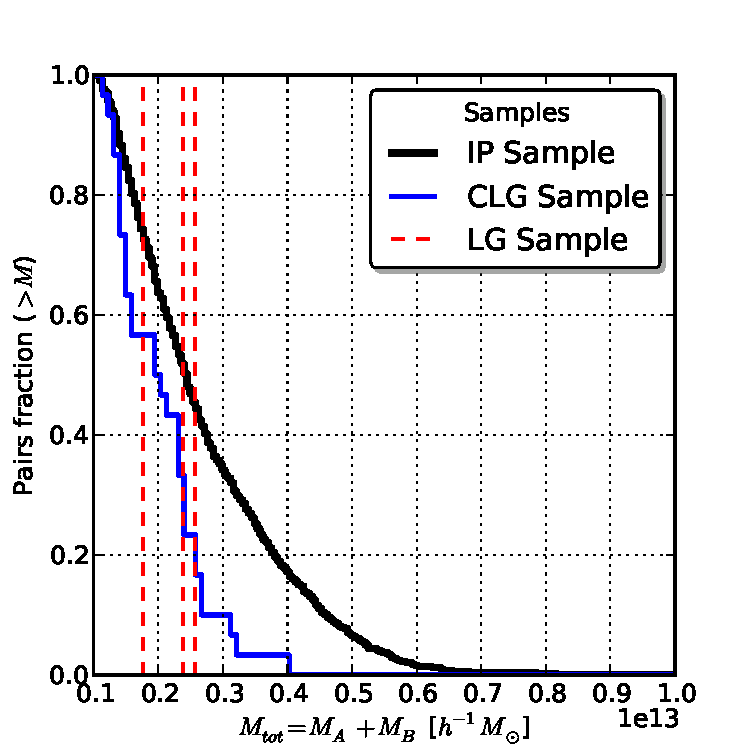
\includegraphics[keepaspectratio=true,width=0.3\textheight]
{./figures/IP_IMF.pdf}
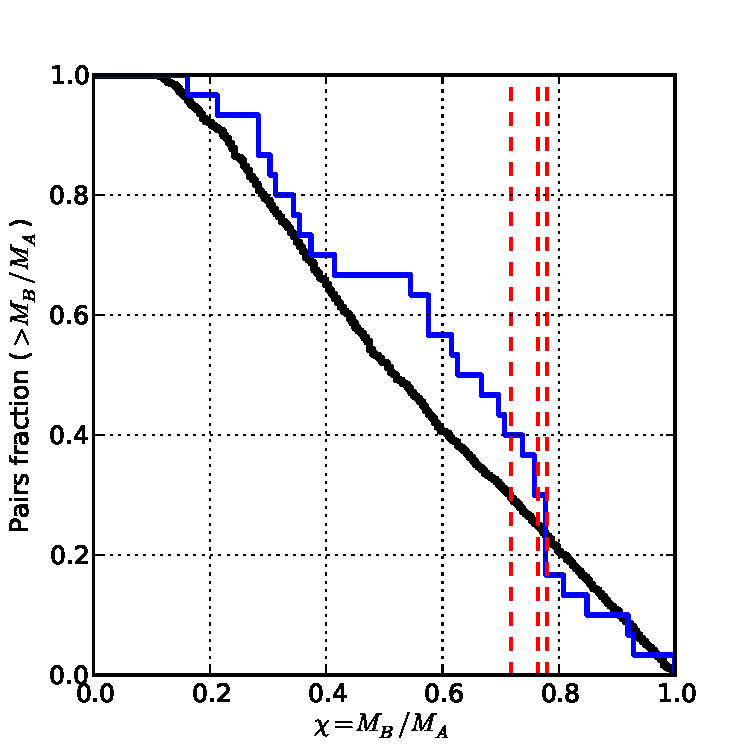
\includegraphics[keepaspectratio=true,width=0.3\textheight]
{./figures/IP_Mass_Ratio.pdf}

\captionof{figure}{\small Integrated distribution of mass ratio index for 
isolated pairs sample (a).}

\label{fig:Index_Pairs}
\vspace{0.1 cm}
\end{center}
\end{flushleft}
%.........................................................................

... Radial vs. tangential velocities

... Angular Momentum

... Total Mechanical energy.

... Reduced Spin


%-------------------------------------------------------------------------
\subsection{Bias induced on the Mass Assembly Histories}
\label{subsec:bias_MAH}
%-------------------------------------------------------------------------

... Last major merger. Formation Time. Assembly Time.

%-------------------------------------------------------------------------
\subsection{Pair Alignment with the Cosmic Web}
\label{subsec:alignment_cosmic_web}
%-------------------------------------------------------------------------

... Separation.

... Relative velocity.

... Angular Momentum.


%*************************************************************************
\section{Conclusions}
\label{sec:conclusions}
%*************************************************************************


%*************************************************************************
\section*{Acknowledgments}  
%*************************************************************************


\bibliographystyle{mn2e}
\bibliography{references} 


\end{document}
